\chapter{Experimentos Realizados}
\thispagestyle{plain}
\label{cap:experimentos}
\graphicspath{{./Cap4_Experimentos_Realizados/Figures/}}

A realização dos experimentos baseou-se na utilização da ferramenta de parametrização e obtenção de métricas, aplicado nas imagens tratadas de cada cena, conforme variaçoes definidas no Capítulo anterior. Os dados obtidos foram organizados de forma a facilitar a análise e comparação entre as variaçoes em cada cena e também entre os diferentes dispositivos sendo testados.

Para cada variação de resolução, que depende de uma nova seleção de parâmetros, será exibido a matriz de resultados final juntamente com as faces detectadas, após já feita a análise para se chegar a um melhor resultado, indicando quais foram os parâmetros definidos.

\section{Cena 1}

\subsection{Otimização de parâmetros}

Primeiramente, foi realizada a otimização dos parâmetros para cada variação de resolução, a partir das imagens com todas as faces disponíveis de cada resolução. No caso desta cena, que exige relativamente muito mais processamento, utilizou-se o Raspberry Pi 4B para a definição dos parâmetros, repetindo-os nos testes com o Raspberry Pi Zero W para base de comparação.

A definição dos parâmetros 'ótimos' não é objetiva. Para esta cena, buscou-se um melhor resultado em que houvesse a maior quantidade de faces detectadas sem a presença de falsos positivos e no menor tempo. Durante a análise, teve-se a razoabilidade de considerar na comparação entre os diferentes resultados da matriz que, um grande aumento no tempo de detecção não justifica um pequeno ganho relativo na quantidade de faces detectadas.

As próximas três subsubseções \ref{sssec:resolution1}, \ref{sssec:resolution2} e \ref{sssec:resolution3} mostram através de imagens, para cada resolução testada, a última iteração da matriz de resultados com os dados entrada, a célula destacada com os parâmetros escolhidos e a imagem com a faces detectadas.

Os parâmetros definidos de cada resolução foram usados para obter as métricas de cada variação de quantidade de faces detectáveis, e em ambos os dispositivos testados. Não será apresentado nesse documento cada resultado das métricas obtidos em tela. Todos os dados foram tabelados e utilizados para as comparações feitas nas subseções seguintes.


\subsubsection{Resolução 1440p} \label{sssec:resolution1}

\begin{figure}[H]
    \centering
    \caption[Otimização Cena1 resolução 1440p.]{Otimização Cena1 resolução 1440p.}
    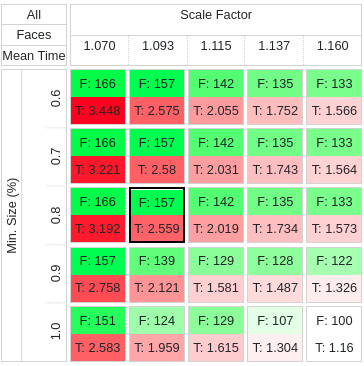
\includegraphics[width=0.85\textwidth]{Cap4_Experimentos_Realizados/Figures/cena1_param_1440p_matriz.jpg}
    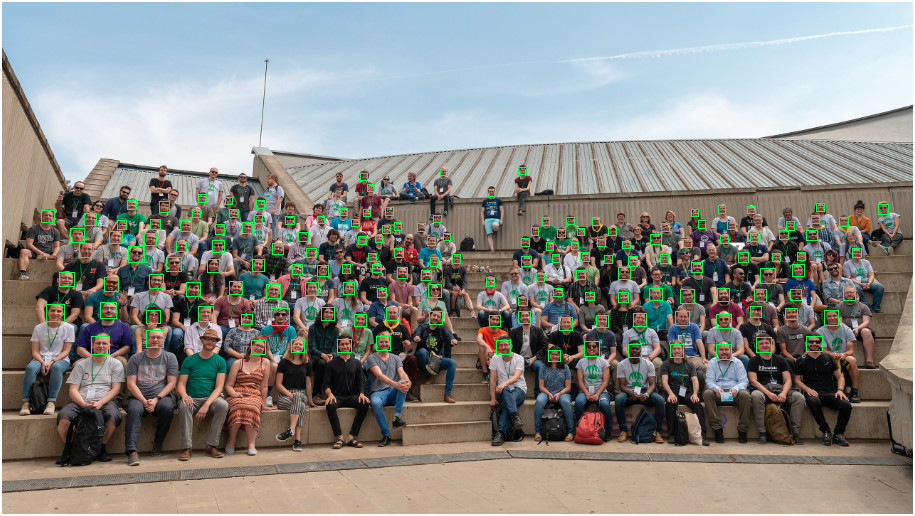
\includegraphics[width=0.85\textwidth]{Cap4_Experimentos_Realizados/Figures/cena1_param_1440p_faces.jpg}
    \caption*{Fonte: autor.}
    \label{fig:otimizacaoCena1_1440p}
\end{figure}

\subsubsection{Resolução 1080p} \label{sssec:resolution2}

\begin{figure}[H]
    \centering
    \caption[Otimização Cena1 resolução 1080p.]{Otimização Cena1 resolução 1080p.}
    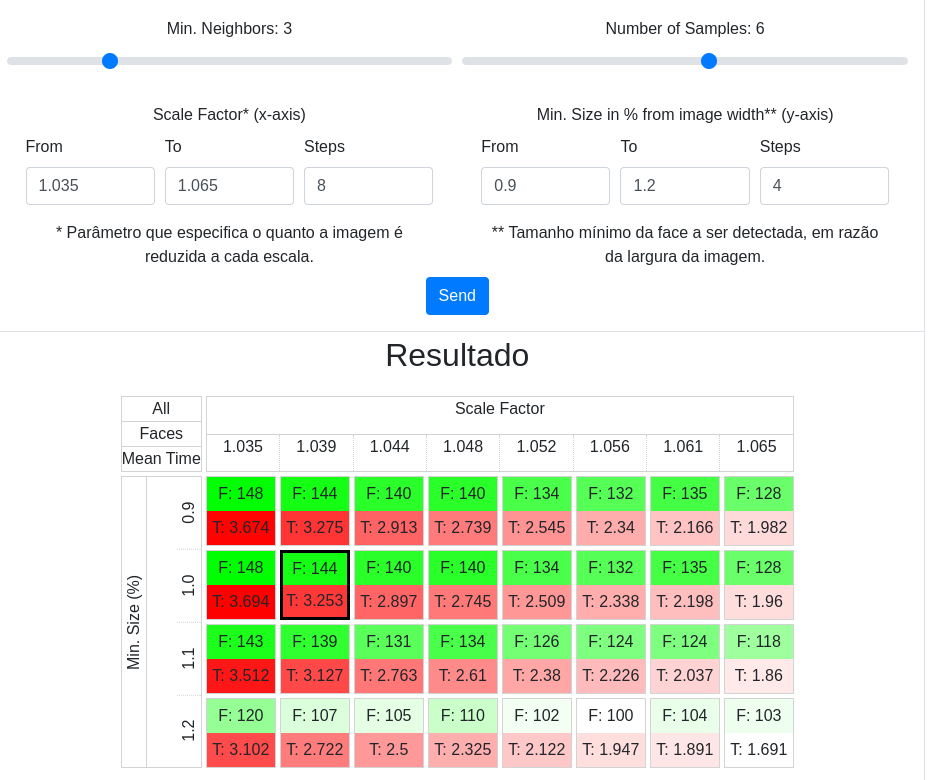
\includegraphics[width=0.85\textwidth]{Cap4_Experimentos_Realizados/Figures/cena1_param_1080p_matriz.jpg}
    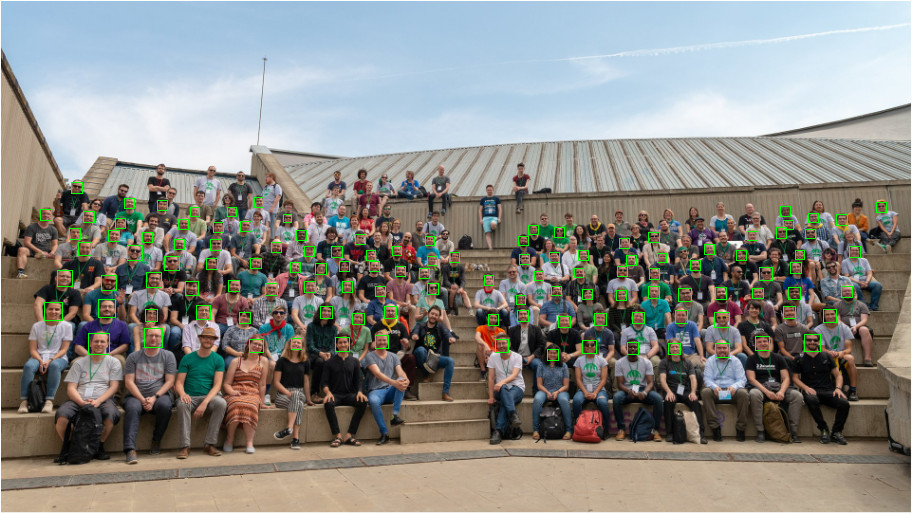
\includegraphics[width=0.85\textwidth]{Cap4_Experimentos_Realizados/Figures/cena1_param_1080p_faces.jpg}
    \caption*{Fonte: autor.}
    \label{fig:otimizacaoCena1_1080p}
\end{figure}

\subsubsection{Resolução 720p} \label{sssec:resolution3}

\begin{figure}[H]
    \centering
    \caption[Otimização Cena1 resolução 720p.]{Otimização Cena1 resolução 720p.}
    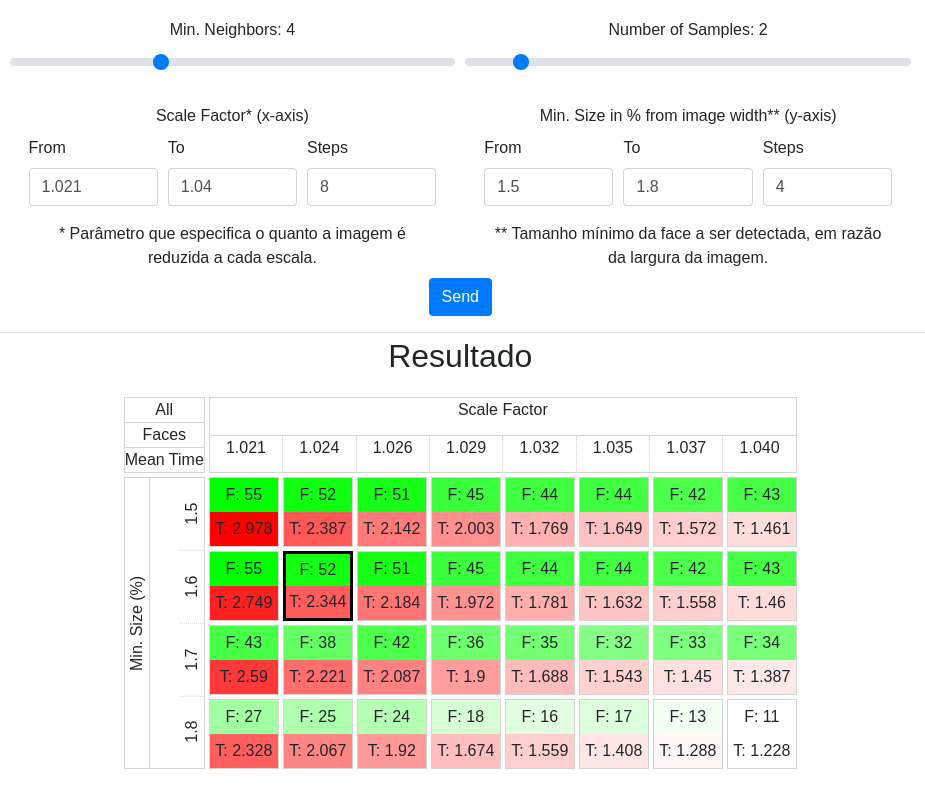
\includegraphics[width=0.85\textwidth]{Cap4_Experimentos_Realizados/Figures/cena1_param_720p_matriz.jpg}
    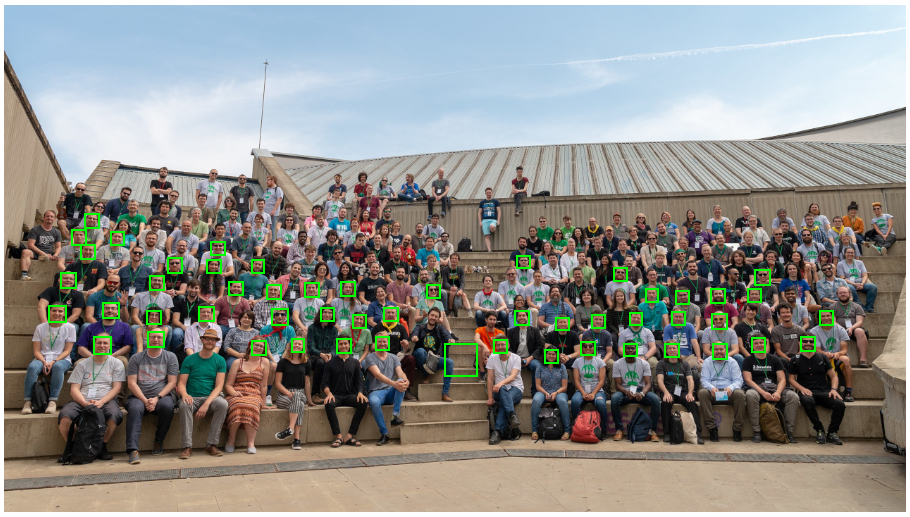
\includegraphics[width=0.85\textwidth]{Cap4_Experimentos_Realizados/Figures/cena1_param_720p_faces.jpg}
    \caption*{Fonte: autor.}
    \label{fig:otimizacaoCena1_720p}
\end{figure}